\documentclass[11pt,a4paper]{article}

% ====================== ENCODAGE / LANGUE ======================
\usepackage[utf8]{inputenc}
\usepackage[T1]{fontenc}
\usepackage[french,provide=*]{babel}

% ====================== MISE EN PAGE ======================
\usepackage[a4paper,margin=2.3cm,headheight=15pt]{geometry}
\usepackage{fancyhdr}
\usepackage{amssymb}
\usepackage{xcolor}
\usepackage{graphicx}
\usepackage{enumitem}
\usepackage{booktabs}
\usepackage{array}
\usepackage{tikz}
\usetikzlibrary{shapes.geometric,arrows.meta,positioning}
\usepackage{listings}
\usepackage[most]{tcolorbox}
\usepackage[hidelinks]{hyperref}
\usepackage{titlesec}

% ====================== COULEURS ======================
\definecolor{cmdbg}{RGB}{31,41,55}       % fond commandes (gris ardoise)
\definecolor{cmdfg}{RGB}{229,231,235}     % texte commandes
\definecolor{outbg}{RGB}{244,245,247}     % fond sorties
\definecolor{outframe}{RGB}{203,213,225}
\definecolor{accent}{RGB}{37,99,235}      % bleu accent
\definecolor{phbg}{RGB}{255,243,224}      % fond placeholder
\definecolor{phframe}{RGB}{234,88,12}     % bord placeholder (orange)
\definecolor{repbg}{RGB}{236,253,245}     % fond reponse (vert clair)
\definecolor{repframe}{RGB}{16,185,129}
\definecolor{notebg}{RGB}{239,246,255}    % fond note (bleu clair)
\definecolor{noteframe}{RGB}{59,130,246}
\definecolor{kw}{RGB}{96,165,250}
\definecolor{cmt}{RGB}{148,163,184}

% ====================== STYLES DE CODE ======================
% Commandes shell : fond sombre
\lstdefinestyle{cmd}{
  backgroundcolor=\color{cmdbg},
  basicstyle=\ttfamily\footnotesize\color{cmdfg},
  breaklines=true,
  breakatwhitespace=false,
  postbreak=\mbox{\textcolor{cmt}{$\hookrightarrow$}\space},
  columns=fullflexible,
  keepspaces=true,
  showstringspaces=false,
  frame=single,
  framesep=5pt,
  rulecolor=\color{cmdbg},
  xleftmargin=4pt,
  xrightmargin=4pt,
  aboveskip=8pt,
  belowskip=4pt,
}
% Sorties OpenSSL : fond clair
\lstdefinestyle{out}{
  backgroundcolor=\color{outbg},
  basicstyle=\ttfamily\scriptsize,
  breaklines=true,
  breakatwhitespace=false,
  postbreak=\mbox{\textcolor{cmt}{$\hookrightarrow$}\space},
  columns=fullflexible,
  keepspaces=true,
  showstringspaces=false,
  frame=single,
  framesep=5pt,
  rulecolor=\color{outframe},
  xleftmargin=4pt,
  xrightmargin=4pt,
  aboveskip=8pt,
  belowskip=8pt,
}
% Fichier de configuration
\lstdefinestyle{conf}{
  backgroundcolor=\color{outbg},
  basicstyle=\ttfamily\scriptsize,
  breaklines=true,
  columns=fullflexible,
  keepspaces=true,
  frame=single,
  framesep=5pt,
  rulecolor=\color{outframe},
  xleftmargin=4pt,
  xrightmargin=4pt,
  commentstyle=\color{cmt}\itshape,
  morecomment=[l]{\#},
}
\lstset{style=cmd}

% ====================== BOITES (placeholder / reponse / note) ======================
\newtcolorbox{placeholder}[1][]{
  colback=phbg, colframe=phframe, coltitle=white,
  fonttitle=\bfseries, title={\faToReplace À COMPLÉTER (non réalisable hors ligne / hors VM)},
  boxrule=1pt, arc=2pt, left=6pt, right=6pt, top=4pt, bottom=4pt, #1}
\newtcolorbox{reponse}[1][]{
  colback=repbg, colframe=repframe, coltitle=white,
  fonttitle=\bfseries, title={Réponse},
  boxrule=1pt, arc=2pt, left=6pt, right=6pt, top=4pt, bottom=4pt, #1}
\newtcolorbox{notebox}[1][]{
  colback=notebg, colframe=noteframe, coltitle=white,
  fonttitle=\bfseries, title={Note},
  boxrule=1pt, arc=2pt, left=6pt, right=6pt, top=4pt, bottom=4pt, #1}
% petit symbole pour le titre placeholder
\newcommand{\faToReplace}{$\blacktriangleright$~}

% ====================== EN-TETES ======================
\pagestyle{fancy}
\fancyhf{}
\fancyhead[L]{\footnotesize TP --- Cryptographie}
\fancyhead[R]{\footnotesize Gestion du cycle de vie des certificats}
\fancyfoot[C]{\thepage}
\renewcommand{\headrulewidth}{0.4pt}
\renewcommand{\footrulewidth}{0pt}

% titres de section colores
\titleformat{\section}{\Large\bfseries\color{accent}}{\thesection}{0.6em}{}
\titleformat{\subsection}{\large\bfseries}{\thesubsection}{0.6em}{}
\titleformat{\subsubsection}{\normalsize\bfseries\color{accent!80!black}}{\thesubsubsection}{0.6em}{}

% macros pratiques
\newcommand{\tri}{\texttt{APV}}
\newcommand{\fichier}[1]{\texttt{#1}}
\newcommand{\cmdinline}[1]{\colorbox{outbg}{\ttfamily\small #1}}

\begin{document}

% ============================================================
%                        PAGE DE TITRE
% ============================================================
\begin{titlepage}
\centering
\vspace*{1.5cm}
{\Large\scshape IMT Mines Alès}\\[0.3cm]
{\large Gestion du cycle de vie des certificats}\\[2cm]

\rule{\linewidth}{0.5pt}\\[0.4cm]
{\Huge\bfseries TP\\[0.3cm]Cryptographie\par}
\vspace{0.4cm}
{\large Construction et exploitation d'une infrastructure de gestion de clés\par}
\rule{\linewidth}{0.5pt}\\[1.5cm]

\end{titlepage}

\tableofcontents
\newpage

% ============================================================
%                     INTRODUCTION GENERALE
% ============================================================
\section{Introduction}

\subsection{Objectifs}
Ce TP se décompose en trois parties :
\begin{itemize}[leftmargin=1.4em]
  \item \textbf{Partie 1 : Étude de certificats existants.} Récupération et analyse
  du certificat TLS du site \url{https://cyber.gouv.fr/}, lecture de la chaîne de
  certification, des extensions, de la CRL, et vérification de statut de révocation
  par CRL puis par OCSP.
  \item \textbf{Partie 2 : Construction d'une PKI multi-autorités.} Mise en place
  d'une hiérarchie inspirée de Let's Encrypt (deux racines, RSA et ECDSA, deux
  autorités subordonnées), avec révocation par CRL et par OCSP, échange S/MIME et
  \emph{certification croisée} entre les deux racines.
  \item \textbf{Partie 3 : Racine adossée à un HSM.} Création d'une autorité racine
  dont la clé privée ne quitte jamais un module cryptographique (HSM virtuel
  SoftHSM2, via PKCS\#11), puis signature d'une autorité subordonnée Microsoft ADCS.
\end{itemize}

\subsection{Choix de dimensionnement (recommandations ANSSI)}

\begin{center}
\renewcommand{\arraystretch}{1.3}
\begin{tabular}{>{\raggedright}p{4.3cm} l l l}
\toprule
\textbf{Entité} & \textbf{Algorithme} & \textbf{Taille / courbe} & \textbf{Hachage}\\
\midrule
\fichier{RSA\_Root\_CA\_\tri} (racine)      & RSA   & 4096 bits     & SHA-256\\
\fichier{Sub\_RSA\_CA\_1\_\tri} (sous-AC)    & RSA   & 3072 bits     & SHA-256\\
\fichier{EC\_Root\_CA\_\tri} (racine)        & ECDSA & secp384r1 (P-384) & SHA-256\\
\fichier{Sub\_EC\_CA\_1\_\tri} (sous-AC)     & ECDSA & secp384r1 (P-384) & SHA-256\\
Entité finale RSA                            & RSA   & 3072 bits     & SHA-256\\
Entité finale EC                             & ECDSA & prime256v1 (P-256) & SHA-256\\
Racine HSM (Partie 3)                        & RSA   & 4096 bits     & SHA-256\\
\bottomrule
\end{tabular}
\end{center}

\subsection{Durées de validité demandées}
\begin{center}
\renewcommand{\arraystretch}{1.2}
\begin{tabular}{l l l}
\toprule
\textbf{Objet} & \textbf{Durée} & \textbf{Valeur \cmdinline{-days} / CRL}\\
\midrule
AC racines            & 15 ans  & \texttt{5479} jours\\
AC subordonnées       & 10 ans  & \texttt{3653} jours\\
Entités finales       & 1 an    & \texttt{365} jours\\
CRL / ARL             & 1 mois  & \texttt{default\_crl\_days = 30}\\
Racine HSM (Partie 3) & 10 ans  & \texttt{3653} jours\\
AC subordonnée ADCS   & 5 ans   & \texttt{1825} jours\\
\bottomrule
\end{tabular}
\end{center}

\newpage

% ============================================================
%                          PARTIE 1
% ============================================================
\section{Partie 1 : Étude de certificats existants}

\subsection{Récupération du certificat (Q1)}

\textbf{Q1. Quel protocole sécurise la connexion dans un navigateur ?}
\begin{reponse}
La connexion HTTPS est sécurisée par TLS. La connexion OpenSSL observée a utilisé TLSv1.3. SSL est l'ancien nom historique, aujourd'hui, le protocole utilisé est TLS.
\end{reponse}

\begin{lstlisting}[style=cmd]
openssl s_client -connect cyber.gouv.fr:443 -servername cyber.gouv.fr -showcerts \
  2>/dev/null </dev/null > cyber.gouv.fr.chain.txt
awk '/BEGIN CERTIFICATE/{c++} END{print c}' cyber.gouv.fr.chain.txt
openssl s_client -connect cyber.gouv.fr:443 -servername cyber.gouv.fr 2>/dev/null </dev/null \
  | openssl x509 -out cyber.gouv.fr.pem
\end{lstlisting}
\begin{lstlisting}[style=out]
2
\end{lstlisting}

\subsection{Lecture de la chaîne (Q2 à Q5)}
\begin{reponse}
\textbf{Q2. Longueur de la chaîne :} la chaîne fournie par \texttt{openssl s\_client}
contient 2 certificats : le certificat serveur \texttt{cyber.gouv.fr} et le
certificat subordonné \texttt{GandiCert}. La racine n'est pas envoyée par le serveur car
elle est supposée présente dans le magasin de confiance du client.\\[4pt]
\textbf{Q3. AC racine :} \texttt{DigiCert Global Root G2}. Elle n'est pas fournie dans
la chaîne TLS récupérée, mais constitue l'ancre de confiance de la chaîne
\texttt{GandiCert}.\\[4pt]
\textbf{Q4. AC subordonnée :} le certificat serveur est émis par
\texttt{C=FR, O=Gandi SAS, CN=GandiCert}.\\[4pt]
\textbf{Q5. Taille de la clé publique du site :} le certificat \texttt{cyber.gouv.fr}
contient une clé publique RSA 4096 bits.
\end{reponse}

\subsection{Analyse du certificat (Q6 à Q16)}
\begin{lstlisting}[style=cmd]
openssl x509 -in cyber.gouv.fr.pem -noout -text > cyber.gouv.fr.x509.txt
\end{lstlisting}

\textbf{Q6. Type de certificat.}
\begin{reponse}
Il s'agit d'un certificat X.509 v3 d'entité finale pour serveur TLS. Le sujet contient
\texttt{CN=cyber.gouv.fr}. Les SAN observés sont \texttt{DNS:cyber.gouv.fr},
\texttt{DNS:ssi.gouv.fr}, \texttt{DNS:www.ssi.gouv.fr} et
\texttt{DNS:www.cyber.gouv.fr}. L'Extended Key Usage contient
\texttt{TLS Web Server Authentication} et les \texttt{Basic Constraints} indiquent
\texttt{CA:FALSE}.
\end{reponse}

\textbf{Q7. Peut-il signer d'autres certificats ?}
\begin{reponse}
\textbf{Non.} Le certificat contient \texttt{Basic Constraints: CA:FALSE}. Son
\texttt{Key Usage} vaut \texttt{Digital Signature, Key Encipherment} et ne contient pas
\texttt{keyCertSign}. Il ne peut donc pas signer d'autres certificats.
\end{reponse}

\textbf{Q8. Peut-il signer du courrier électronique ?}
\begin{reponse}
\textbf{Non pour l'usage S/MIME.} L'Extended Key Usage contient uniquement
\texttt{TLS Web Server Authentication} et ne contient pas \texttt{E-mail Protection}
(\texttt{emailProtection}).
\end{reponse}

\textbf{Q9. Où trouve-t-on la CRL de l'AC émettrice ?}
\begin{reponse}
Les points de distribution CRL réellement présents sont :
\begin{lstlisting}[style=out]
http://crl3.digicert.com/GandiCert.crl
http://crl4.digicert.com/GandiCert.crl
\end{lstlisting}
\end{reponse}

\textbf{Q10. Format du numéro de série et conversion décimale.}
\begin{reponse}
Le numéro de série est affiché en hexadécimal par OpenSSL.
\begin{lstlisting}[style=out]
Serial hex avec separateurs : 05:7e:1f:dd:c4:8e:7a:07:80:64:3a:be:eb:cc:52:a5
Serial hex normalise       : 057E1FDDC48E7A0780643ABEEBCC52A5
Serial decimal             : 7301015708052902158374241928634716837
\end{lstlisting}
Il s'agit d'un entier ASN.1 affiché en hexadécimal, la valeur décimale montre qu'il
s'agit d'un grand nombre non trivial à prédire.
\end{reponse}

\textbf{Q11. Afficher la clé publique.}
\begin{lstlisting}[style=cmd]
openssl x509 -in cyber.gouv.fr.pem -pubkey -noout
\end{lstlisting}
\begin{lstlisting}[style=out]
Public Key Algorithm: rsaEncryption
Public-Key: (4096 bit)
Exponent: 65537 (0x10001)
\end{lstlisting}

\textbf{Q12. Afficher la clé privée.}
\begin{reponse}
C'est impossible à partir du certificat public. Un certificat X.509 contient la clé
publique, l'identité, les extensions et la signature de l'autorité, mais jamais la clé
privée. Celle-ci reste uniquement côté serveur.
\end{reponse}

\textbf{Q13 à Q16. Lecture et vérification de la CRL.}
\begin{lstlisting}[style=cmd]
wget -O GandiCert.crl http://crl3.digicert.com/GandiCert.crl
openssl crl -inform DER -in GandiCert.crl -text -noout > crl.txt
rg "057E1FDDC48E7A0780643ABEEBCC52A5|05:7E:1F:DD:C4:8E:7A:07:80:64:3A:BE:EB:CC:52:A5" crl.txt
\end{lstlisting}
\begin{reponse}
\textbf{Q13.} La CRL consultée indique :
\begin{lstlisting}[style=out]
Last Update: Jun 22 12:45:56 2026 GMT
Next Update: Jun 29 12:45:56 2026 GMT
\end{lstlisting}
Sa durée de validité est donc de 7 jours.\\[4pt]
\textbf{Q14.} Les premières entrées affichées dans \texttt{crl.txt} ne montrent que le
numéro de série et la date de révocation. Des champs \texttt{X509v3 CRL Reason Code}
apparaissent plus loin, mais pas systématiquement pour les premières entrées.\\[4pt]
\textbf{Q15.} Pour vérifier rapidement que la CRL est la bonne, on contrôle que son
\texttt{Issuer} correspond à l'AC émettrice du certificat
(\texttt{C=FR, O=Gandi SAS, CN=GandiCert}), que l'URL provient bien des
\texttt{CRL Distribution Points}, puis que la signature de la CRL est vérifiable avec
le certificat de cette AC.\\[4pt]
\textbf{Q16.} La recherche du numéro de série du certificat \texttt{cyber.gouv.fr} dans
la CRL ne renvoie aucun résultat : le certificat n'apparaît donc pas comme révoqué dans
la CRL consultée.
\end{reponse}

\subsection{La révocation (Q17 à Q21)}

\textbf{Site \texttt{https://revoked-rsa-dv.ssl.com/} dans 3 navigateurs.}
\begin{figure}[htbp]
  \centering
  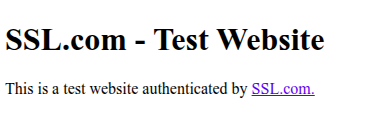
\includegraphics[width=0.48\linewidth]{images/revoked_rsa_chrome.png}\hfill
  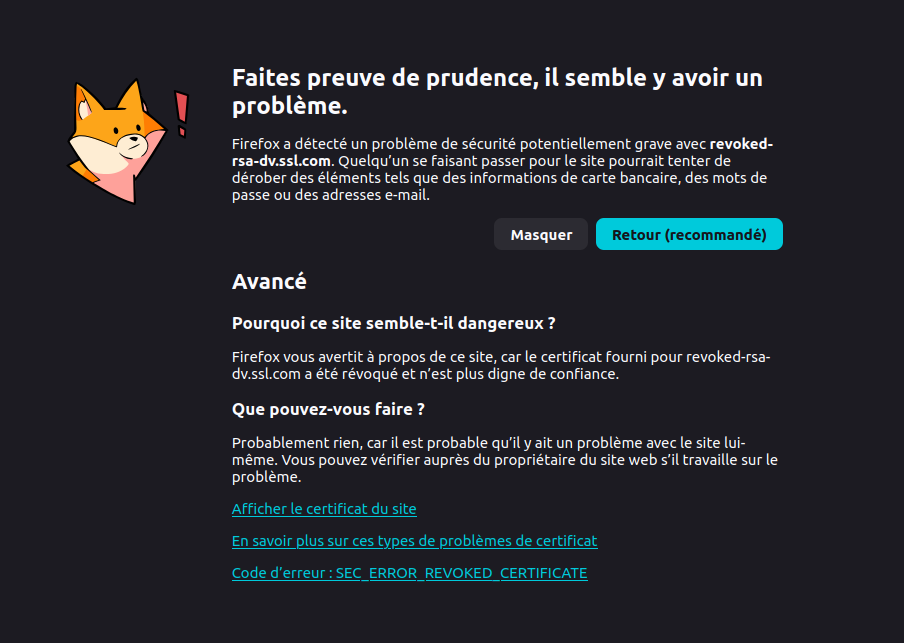
\includegraphics[width=0.48\linewidth]{images/revoked_rsa_firefox.png}
  \caption{Pages d'erreur de sécurité pour \url{https://revoked-rsa-dv.ssl.com} : à gauche Chrome, à droite Firefox.}
  \label{fig:revoked-browsers}
\end{figure}

\textbf{Q17. Le série du certificat révoqué est-il dans la CRL ?}
\begin{reponse}
Oui. Le certificat testé est \texttt{01-public-certs/revoked-rsa-dv.ssl.com.pem}. Son
numéro de série est :
\begin{lstlisting}[style=out]
1811B09C4BB9E179133BB9D9A9B140C5
\end{lstlisting}
La CRL utilisée est \texttt{http://crls.ssl.com/SSL.com-TLS-I-RSA-R1.crl}. Le numéro y
apparaît avec la date de révocation suivante :
\begin{lstlisting}[style=out]
Serial Number: 1811B09C4BB9E179133BB9D9A9B140C5
Revocation Date: Jun  9 14:37:38 2026 GMT
\end{lstlisting}
\end{reponse}

\textbf{Q18. Vérification OCSP.}
\begin{lstlisting}[style=cmd]
openssl ocsp \
  -issuer ssl.com-tls-i-rsa-r1.pem \
  -cert revoked-rsa-dv.ssl.com.pem \
  -url http://ocsps.ssl.com \
  -no_nonce \
  -resp_text -text
\end{lstlisting}
\begin{lstlisting}[style=out]
OCSP Response Status: successful (0x0)
Cert Status: revoked
Revocation Time: Jun  9 14:37:38 2026 GMT
revoked-rsa-dv.ssl.com.pem: revoked
\end{lstlisting}
\begin{reponse}
La CRL et OCSP concordent : le certificat est bien révoqué.
\end{reponse}

\textbf{Q19. Numéros de série de \texttt{google.com} et \texttt{youtube.com}.}
\begin{lstlisting}[style=out]
google.com  : 139CDF29A8B5BC5212413EEEAFD18CBE
youtube.com : 139CDF29A8B5BC5212413EEEAFD18CBE
\end{lstlisting}
\begin{reponse}
Les deux hôtes ont présenté le même certificat feuille, émis par
\texttt{C=US, O=Google Trust Services, CN=WR2}, avec \texttt{CN=*.google.com}. Les SAN
contiennent à la fois \texttt{DNS:google.com} et \texttt{DNS:youtube.com}. Il s'agit
donc d'un certificat multi-SAN partagé par l'infrastructure Google.
\end{reponse}

\textbf{Q20. \texttt{https://wrong.host.badssl.com/}.}
\begin{lstlisting}[style=out]
verify error:num=62:hostname mismatch
Verification error: hostname mismatch
\end{lstlisting}
\begin{reponse}
L'alerte est cohérente : le nom demandé \texttt{wrong.host.badssl.com} ne correspond pas
au certificat présenté. La validation du nom d'hôte repose sur les SAN, ou à défaut sur
le CN selon la logique de la RFC 6125. Un wildcard ne couvre qu'un seul niveau de
sous-domaine.
\end{reponse}

\textbf{Q21. Certificats racines ISRG.}
\begin{reponse}
Non réalisé car on a pas les fichiers \texttt{isrg-1.crt} et \texttt{isrg-2.crt}. La méthode de lecture reste :
\begin{lstlisting}[style=cmd]
for f in isrg-1.crt isrg-2.crt; do
  openssl x509 -in $f -noout -subject -issuer -dates
  openssl x509 -in $f -noout -text | grep -E "Public Key Algorithm|Public-Key|Signature Algorithm"
done
\end{lstlisting}
\end{reponse}

\newpage
% ============================================================
%                          PARTIE 2
% ============================================================
\section{Partie 2 : Construction d'une PKI multi-autorités}

\subsection{La certification croisée n'est que dans un sens}
\begin{reponse}
\textbf Une certification croisée consiste à
faire signer la clé publique d'une racine par l'autre racine, ce qui produit un
certificat supplémentaire pour la même autorité. Ici, \texttt{RSA\_Root\_CA\_\tri}
signe un certificat croisé pour \texttt{EC\_Root\_CA\_\tri}. Un vérificateur qui fait
confiance à la racine RSA peut donc valider une chaîne de la branche EC via ce certificat
croisé. L'inverse n'est pas vrai sans certificat miroir
\texttt{RSA\_Root\_CA\_\tri} signé par \texttt{EC\_Root\_CA\_\tri}.
\end{reponse}

\begin{reponse}
\textbf{Exemple de chaîne croisée unidirectionnelle :}
\begin{lstlisting}[style=out]
RSA_Root_CA_APV
  -> EC_Root_CA_APV (certificat croise signe par RSA_Root_CA_APV)
  -> Sub_EC_CA_1_APV
  -> Leaf_EC_1_APV.crosspath
\end{lstlisting}
\textbf{Pour une certification croisée dans les deux sens}, il faudrait émettre un
second certificat croisé, cette fois avec la racine EC comme émetteur et la clé publique
de la racine RSA comme sujet :
\begin{lstlisting}[style=out]
RSA_Root_CA_APV -> EC_Root_CA_APV
EC_Root_CA_APV  -> RSA_Root_CA_APV
\end{lstlisting}
\end{reponse}

\subsection{Tâche 1 : Méthodologie de mise en place}

\subsubsection{Arborescence dédiée et fichiers de base de données}
Chaque AC dispose de son répertoire, avec \fichier{private/} (clé privée, \texttt{chmod
700}) et \fichier{db/} (base de données OpenSSL).

\begin{lstlisting}[style=cmd]
mkdir -p ca/{certs,crl,newcerts,csr,smime,ocsp}
for CA in RSA_Root_CA EC_Root_CA Sub_RSA_CA_1 Sub_EC_CA_1; do
  mkdir -p ca/$CA/db ca/$CA/private
  chmod 700 ca/$CA/private
  : > ca/$CA/db/$CA.db            # base vide mais existante
  : > ca/$CA/db/$CA.db.attr
  echo 01 > ca/$CA/db/$CA.srl     # numero de serie initial
  echo 01 > ca/$CA/db/$CA.crl.srl # numero de CRL initial
done
\end{lstlisting}

\subsubsection{Fichier de configuration OpenSSL (un par AC)}
Extrait de la configuration de la
racine RSA (\fichier{RSA\_Root\_CA.conf}) :
\begin{lstlisting}[style=conf]
[ca]
default_ca = root_ca

[root_ca]
certificate      = $dir/RSA_Root_CA.crt
private_key      = $dir/private/RSA_Root_CA.key
database         = $dir/db/RSA_Root_CA.db
serial           = $dir/db/RSA_Root_CA.srl
crlnumber        = $dir/db/RSA_Root_CA.crl.srl
default_md       = sha256          # hachage SHA-256 (ANSSI)
default_crl_days = 30              # CRL valable 1 mois
policy           = policy_loose

# --- profil de la racine elle-meme (auto-signature) ---
[root_ca_ext]
basicConstraints       = critical,CA:TRUE,pathlen:2   # 2 niveaux de sous-AC
keyUsage               = critical,keyCertSign,cRLSign
subjectKeyIdentifier   = hash
authorityKeyIdentifier = keyid:always

# --- profil applique aux AC subordonnees signees par la racine ---
[sub_ca_ext]
basicConstraints       = critical,CA:TRUE,pathlen:0   # ne signe que des EE
keyUsage               = critical,keyCertSign,cRLSign
crlDistributionPoints  = URI:http://crl.pki-apv.local/RSA_Root_CA.crl
authorityInfoAccess    = caIssuers;URI:http://aia.pki-apv.local/RSA_Root_CA.crt
\end{lstlisting}

\subsubsection{Création de la racine RSA (auto-signée)}
La requête est créée \emph{et} la bi-clé RSA générée en une commande, puis la racine
s'auto-signe :
\begin{lstlisting}[style=cmd]
# 1) genere la bi-cle RSA 4096 + la CSR
openssl req -new -config ca/RSA_Root_CA/RSA_Root_CA.conf \
  -newkey rsa:4096 -keyout ca/RSA_Root_CA/private/RSA_Root_CA.key -nodes \
  -out ca/csr/RSA_Root_CA.csr
# 2) auto-signature (15 ans, extensions racine)
openssl ca -batch -config ca/RSA_Root_CA/RSA_Root_CA.conf -selfsign \
  -in ca/csr/RSA_Root_CA.csr -extensions root_ca_ext -days 5479 \
  -out ca/RSA_Root_CA/RSA_Root_CA.crt
\end{lstlisting}
Vérification du certificat racine obtenu :
\begin{lstlisting}[style=out]
$ openssl x509 -in RSA_Root_CA.crt -noout -subject -issuer -dates
subject= C = FR, O = TP IMT Mines Ales, OU = PKI APV, CN = RSA Root CA APV
issuer = C = FR, O = TP IMT Mines Ales, OU = PKI APV, CN = RSA Root CA APV
notBefore=Jun 23 06:30:04 2026 GMT
notAfter =Jun 23 06:30:04 2041 GMT          # 15 ans
    X509v3 Basic Constraints: critical
        CA:TRUE, pathlen:2
    X509v3 Key Usage: critical
        Certificate Sign, CRL Sign
\end{lstlisting}

\subsubsection{Création de la racine ECDSA (auto-signée)}
OpenSSL ne génère pas la clé EC implicitement via \texttt{req} : on crée d'abord la clé
P-384, puis la requête, puis l'auto-signature.
\begin{lstlisting}[style=cmd]
# 1) cle EC P-384 (secp384r1)
openssl genpkey -algorithm EC -pkeyopt ec_paramgen_curve:secp384r1 \
  -out ca/EC_Root_CA/private/EC_Root_CA.key
# 2) CSR a partir de la cle existante
openssl req -new -config ca/EC_Root_CA/EC_Root_CA.conf \
  -key ca/EC_Root_CA/private/EC_Root_CA.key -out ca/csr/EC_Root_CA.csr
# 3) auto-signature (15 ans, pathlen:1)
openssl ca -batch -config ca/EC_Root_CA/EC_Root_CA.conf -selfsign \
  -in ca/csr/EC_Root_CA.csr -extensions root_ca_ext -days 5479 \
  -out ca/EC_Root_CA/EC_Root_CA.crt
\end{lstlisting}
\begin{lstlisting}[style=out]
$ openssl x509 -in EC_Root_CA.crt -noout -text | grep -E "Algorithm|NIST|pathlen|Sign"
        Signature Algorithm: ecdsa-with-SHA256
                ASN1 OID: secp384r1
                NIST CURVE: P-384
            CA:TRUE, pathlen:1
            Certificate Sign, CRL Sign
\end{lstlisting}

\subsubsection{Création des autorités subordonnées}
Chaque sous-AC génère sa clé et sa CSR, puis est signée par sa racine avec le profil
\texttt{sub\_ca\_ext} (10 ans). Exemple pour la branche RSA :
\begin{lstlisting}[style=cmd]
openssl req -new -config ca/Sub_RSA_CA_1/Sub_RSA_CA_1.conf \
  -newkey rsa:3072 -keyout ca/Sub_RSA_CA_1/private/Sub_RSA_CA_1.key -nodes \
  -out ca/csr/Sub_RSA_CA_1.csr
# signature par la racine RSA
openssl ca -batch -config ca/RSA_Root_CA/RSA_Root_CA.conf \
  -extensions sub_ca_ext -days 3653 \
  -in ca/csr/Sub_RSA_CA_1.csr -out ca/Sub_RSA_CA_1/Sub_RSA_CA_1.crt
\end{lstlisting}
Validation des deux chaînes de subordination :
\begin{lstlisting}[style=out]
$ openssl verify -CAfile RSA_Root_CA.crt Sub_RSA_CA_1.crt
Sub_RSA_CA_1.crt: OK
$ openssl verify -CAfile EC_Root_CA.crt  Sub_EC_CA_1.crt
Sub_EC_CA_1.crt: OK
\end{lstlisting}

\newpage

\subsection{Révocation par CRL (tâches 2 à 4)}

\textbf{Tâche 2 : émettre une entité finale par \texttt{Sub\_RSA\_CA\_1\_\tri}.}
Le certificat généré se trouve dans le dossier \fichier{03-crl-ocsp} :
\fichier{Sub\_RSA\_CA\_1\_\tri-leaf-crl.crt}.
\begin{lstlisting}[style=cmd]
cd /home/aurelien/Documents/certificats/03-crl-ocsp
openssl ca -batch \
  -config openssl-rsa-sub-ocsp.cnf \
  -extensions v3_leaf \
  -days 365 \
  -notext \
  -in Sub_RSA_CA_1_APV-leaf-crl.csr.pem \
  -out Sub_RSA_CA_1_APV-leaf-crl.crt
\end{lstlisting}

\textbf{Tâche 3 : valider face à la chaîne d'autorité.}
\begin{lstlisting}[style=cmd]
openssl verify \
  -CAfile /home/aurelien/Documents/certificats/02-pki-openssl/RSA_Root_CA_APV/certs/RSA_Root_CA_APV.crt \
  -untrusted /home/aurelien/Documents/certificats/02-pki-openssl/Sub_RSA_CA_1_APV/certs/Sub_RSA_CA_1_APV.crt \
  Sub_RSA_CA_1_APV-leaf-crl.crt
\end{lstlisting}
\begin{lstlisting}[style=out]
/home/aurelien/Documents/certificats/03-crl-ocsp/Sub_RSA_CA_1_APV-leaf-crl.crt: OK
\end{lstlisting}

\textbf{Tâche 4 : révoquer puis générer et afficher la CRL.}
\begin{lstlisting}[style=cmd]
openssl ca -batch -config openssl-rsa-sub-ocsp.cnf \
  -revoke Sub_RSA_CA_1_APV-leaf-crl.crt \
  -crl_reason keyCompromise
openssl ca -config openssl-rsa-sub-ocsp.cnf \
  -gencrl -crldays 30 \
  -out ca-work/Sub_RSA_CA_1_APV/crl.pem
openssl crl -in ca-work/Sub_RSA_CA_1_APV/crl.pem -text -noout > crl-after-revoke.txt
\end{lstlisting}
\begin{lstlisting}[style=out]
Issuer: C=FR, O=TP Crypto Agents, OU=PKI OpenSSL, CN=Sub_RSA_CA_1_APV
Last Update: Jun 23 07:18:21 2026 GMT
Next Update: Jul 23 07:18:21 2026 GMT
Serial Number: 1000
Revocation Date: Jun 23 07:18:21 2026 GMT
X509v3 CRL Reason Code: Key Compromise
\end{lstlisting}
Le certificat apparaît bien dans la CRL, avec le motif \emph{Key Compromise}.


\subsection{Signature et chiffrement S/MIME (tâches 5 à 7)}

\textbf{Tâche 5 : certificat S/MIME avec les bons usages.}
Le certificat \fichier{04-smime/smime-user.crt} est émis par
\texttt{Sub\_RSA\_CA\_1\_\tri}. Les extensions observées sont :
\begin{itemize}[leftmargin=1.4em]
  \item \texttt{Basic Constraints: CA:FALSE} ;
  \item \texttt{Key Usage: Digital Signature, Key Encipherment} ;
  \item \texttt{Extended Key Usage: E-mail Protection} ;
  \item SAN email : \texttt{smime-user@apv.local}.
\end{itemize}
\begin{lstlisting}[style=cmd]
cd /home/aurelien/Documents/certificats/04-smime
openssl ca -batch \
  -config ../02-pki-openssl/Sub_RSA_CA_1_APV/openssl-rsa-sub.cnf \
  -extfile smime-openssl.cnf \
  -extensions v3_smime_signer \
  -days 365 \
  -notext \
  -in smime-user.csr.pem \
  -out smime-user.crt
\end{lstlisting}

\textbf{Tâches 6 et 7 : signature, chiffrement, déchiffrement et vérification.}
Une démo locale a été
réalisée avec un certificat destinataire de test : \fichier{recipient-test.crt}.
\begin{lstlisting}[style=cmd]
openssl smime -sign -binary -nodetach \
  -in message.txt \
  -signer smime-user.crt \
  -inkey smime-user.key.pem \
  -certfile ../02-pki-openssl/Sub_RSA_CA_1_APV/certs/Sub_RSA_CA_1_APV.crt \
| openssl smime -encrypt -aes256 \
  -out signed-encrypted-message.pem \
  recipient-test.crt

openssl smime -decrypt \
  -in signed-encrypted-message.pem \
  -recip recipient-test.crt \
  -inkey recipient-test.key.pem \
  -out decrypted-signed-message.pem

openssl smime -verify \
  -in decrypted-signed-message.pem \
  -CAfile ../02-pki-openssl/RSA_Root_CA_APV/certs/RSA_Root_CA_APV.crt \
  -out verified-message.txt
\end{lstlisting}
\begin{reponse}
Le fichier \fichier{verified-message.txt} contient le message clair attendu.
\end{reponse}


\subsection{Révocation par OCSP (tâches 8 à 12)}

\textbf{Tâche 8 : certificat contenant URL CRL et URL OCSP.}
Le certificat testé se trouve dans le dossier \fichier{03-crl-ocsp} :
\fichier{Sub\_RSA\_CA\_1\_\tri-leaf-ocsp.crt}.
\begin{lstlisting}[style=out]
CRL Distribution Points:
  URI:http://crl.localhost:2560/Sub_RSA_CA_1_APV.crl
Authority Information Access:
  OCSP - URI:http://ocsp.localhost:2560
\end{lstlisting}

\textbf{Tâche 9 : répondeur OCSP pour \texttt{Sub\_RSA\_CA\_1\_\tri}.}
Le répondeur local est lancé sur \texttt{127.0.0.1:2560}.
\begin{lstlisting}[style=cmd]
openssl ocsp \
  -index ca-work/Sub_RSA_CA_1_APV/db/index.txt \
  -port 2560 \
  -rsigner ../02-pki-openssl/Sub_RSA_CA_1_APV/certs/Sub_RSA_CA_1_APV.crt \
  -rkey ../02-pki-openssl/Sub_RSA_CA_1_APV/private/Sub_RSA_CA_1_APV.key.pem \
  -CA ../02-pki-openssl/Sub_RSA_CA_1_APV/certs/Sub_RSA_CA_1_APV.crt \
  -nrequest 1
\end{lstlisting}

\textbf{Tâche 10 : vérifier : statut attendu \emph{good}.}
\begin{lstlisting}[style=cmd]
openssl ocsp \
  -issuer ../02-pki-openssl/Sub_RSA_CA_1_APV/certs/Sub_RSA_CA_1_APV.crt \
  -cert Sub_RSA_CA_1_APV-leaf-ocsp.crt \
  -url http://127.0.0.1:2560 \
  -CAfile ../02-pki-openssl/RSA_Root_CA_APV/certs/RSA_Root_CA_APV.crt \
  -verify_other ../02-pki-openssl/Sub_RSA_CA_1_APV/certs/Sub_RSA_CA_1_APV.crt \
  -resp_text -text -no_nonce
\end{lstlisting}
\begin{lstlisting}[style=out]
Cert Status: good
Response verify OK
Sub_RSA_CA_1_APV-leaf-ocsp.crt: good
\end{lstlisting}

\textbf{Tâches 11 et 12 : révoquer puis re-vérifier : statut attendu \emph{revoked}.}
\begin{lstlisting}[style=cmd]
openssl ca -batch -config openssl-rsa-sub-ocsp.cnf \
  -revoke Sub_RSA_CA_1_APV-leaf-ocsp.crt \
  -crl_reason cessationOfOperation
\end{lstlisting}
\begin{lstlisting}[style=out]
Cert Status: revoked
Revocation Time: Jun 23 07:18:22 2026 GMT
Response verify OK
Sub_RSA_CA_1_APV-leaf-ocsp.crt: revoked
\end{lstlisting}
Le statut passe bien de \texttt{good} à \texttt{revoked}.


\subsection{Certification croisée (tâches 13 et 14)}
\label{sec:cross}

\textbf{Tâche 13 : entité finale émise par \texttt{Sub\_EC\_CA\_1\_\tri}.}
Le certificat final émis pour tester les chemins est
\fichier{05-cross-cert/certs/Leaf\_EC\_1\_\tri.crosspath.crt}.

\textbf{Mise en place du pont croisé.} La racine \texttt{RSA\_Root\_CA\_\tri} signe un
certificat croisé pour \texttt{EC\_Root\_CA\_\tri}. On obtient ainsi un second
certificat pour la racine EC, mais émis par la racine RSA :
\begin{lstlisting}[style=out]
05-cross-cert/certs/EC_Root_CA_APV.cross-signed-by-RSA_Root_CA_APV.crt
\end{lstlisting}

\textbf{Tâche 14 : vérifier les deux chaînes possibles.}
\begin{lstlisting}[style=cmd]
# Chaine native : Leaf_EC -> Sub_EC_CA_1 -> EC_Root_CA
openssl verify -show_chain \
  -CAfile /home/aurelien/Documents/certificats/02-pki-openssl/EC_Root_CA_APV/certs/EC_Root_CA_APV.crt \
  -untrusted /home/aurelien/Documents/certificats/02-pki-openssl/Sub_EC_CA_1_APV/certs/Sub_EC_CA_1_APV.crt \
  /home/aurelien/Documents/certificats/05-cross-cert/certs/Leaf_EC_1_APV.crosspath.crt

# Chaine croisee : Leaf_EC -> Sub_EC_CA_1 -> EC_Root_CA cross-signee -> RSA_Root_CA
openssl verify -show_chain \
  -CAfile /home/aurelien/Documents/certificats/02-pki-openssl/RSA_Root_CA_APV/certs/RSA_Root_CA_APV.crt \
  -untrusted /home/aurelien/Documents/certificats/05-cross-cert/certs/untrusted-rsa-path.pem \
  /home/aurelien/Documents/certificats/05-cross-cert/certs/Leaf_EC_1_APV.crosspath.crt
\end{lstlisting}
\begin{lstlisting}[style=out]
/home/aurelien/Documents/certificats/05-cross-cert/certs/Leaf_EC_1_APV.crosspath.crt: OK
depth=0: CN=Leaf_EC_1_APV
depth=1: CN=Sub_EC_CA_1_APV
depth=2: CN=EC_Root_CA_APV

/home/aurelien/Documents/certificats/05-cross-cert/certs/Leaf_EC_1_APV.crosspath.crt: OK
depth=0: CN=Leaf_EC_1_APV
depth=1: CN=Sub_EC_CA_1_APV
depth=2: CN=EC_Root_CA_APV
depth=3: CN=RSA_Root_CA_APV
\end{lstlisting}


\subsection{Magasin de certificats Windows (tâche 15)}
\label{sec:winstore}

\subsubsection{Pourquoi un « magasin » de certificats}
Sous Linux, on valide une chaîne en désignant explicitement le fichier de l'AC de
confiance (\cmdinline{openssl verify -CAfile racine.crt}). Windows fonctionne autrement :
il ne lit pas des fichiers \fichier{.crt} en vrac, il s'appuie sur des \emph{magasins de
certificats} (\emph{certificate stores}), c'est-à-dire des bases internes du système
rangées par \emph{usage}. Pour qu'un certificat émis par notre PKI soit reconnu comme
valide par Windows, il faut donc \emph{importer} nos certificats dans les bons magasins.

Deux magasins nous intéressent, et la distinction est essentielle :
\begin{itemize}[leftmargin=1.4em]
  \item \textbf{Autorités de certification racines de confiance}
  (chemin PowerShell \texttt{Cert:\textbackslash LocalMachine\textbackslash Root}) : ce
  sont les \emph{ancres de confiance}. Toute chaîne qui remonte jusqu'à une racine placée
  ici est jugée fiable par le système. On n'y met \emph{que} des racines auto-signées.
  \item \textbf{Autorités de certification intermédiaires}
  (\texttt{Cert:\textbackslash LocalMachine\textbackslash CA}) : on y place les AC
  \emph{subordonnées}. Elles ne sont pas des ancres de confiance ; elles servent à
  Windows pour reconstruire le chemin entre un certificat d'entité finale et la racine.
\end{itemize}

\begin{notebox}
\texttt{LocalMachine} désigne le magasin de \emph{l'ordinateur} (valable pour tous les
comptes et pour les services comme IIS) ; \texttt{CurrentUser} ne concernerait que la
session courante. Pour une PKI de serveur, on importe toujours dans
\texttt{LocalMachine}, ce qui exige une console PowerShell \textbf{en administrateur}.
\end{notebox}

\subsubsection{Certificats à importer}
On illustre ici avec la chaîne de la Partie~3 (racine adossée au HSM) :
\begin{itemize}[leftmargin=1.4em]
  \item racine : \fichier{rootCA.crt} (\texttt{CN=RootCA}, auto-signée, à mettre dans
  \texttt{Root}) ;
  \item intermédiaire : le certificat de l'AC subordonnée ADCS \fichier{sub\_ca.crt}
  (\texttt{CN=Sub-ADCS-CA-APV}, à mettre dans \texttt{CA}).
\end{itemize}
La même méthode s'applique à la chaîne OpenSSL de la Partie~2
(\fichier{RSA\_Root\_CA\_\tri.crt} en racine, \fichier{Sub\_RSA\_CA\_1\_\tri.crt} en
intermédiaire).

\subsubsection{Import dans les magasins (PowerShell administrateur)}
\begin{lstlisting}[style=cmd]
# Racine HSM -> magasin des racines de confiance de la machine
Import-Certificate -FilePath C:\TP-Crypto-ADCS\input\rootCA.crt `
  -CertStoreLocation Cert:\LocalMachine\Root

# AC subordonnee ADCS -> magasin des AC intermediaires
Import-Certificate -FilePath C:\TP-Crypto-ADCS\input\sub_ca.crt `
  -CertStoreLocation Cert:\LocalMachine\CA
\end{lstlisting}

\begin{notebox}
L'équivalent en ligne de commande historique est \cmdinline{certutil -addstore Root
rootCA.crt} et \cmdinline{certutil -addstore CA sub\_ca.crt}. C'est d'ailleurs ce qui a été
utilisé en Partie~3 ; l'import effectif de la racine dans le magasin \texttt{Root} est
visible figure~\ref{fig:adcs-rootstore}.
\end{notebox}

\subsubsection{Vérification de la chaîne}
Deux contrôles complémentaires :
\begin{lstlisting}[style=cmd]
# 1) Inspection graphique : ouvrir la console des certificats machine
certlm.msc
# Double-cliquer le certificat, onglet "Chemin d'acces de certification".

# 2) Verification en ligne de commande de la chaine
certutil -verify C:\TP-Crypto-ADCS\input\sub_ca.crt
\end{lstlisting}
\begin{reponse}
Résultat (cf. Partie~3) : dans l'onglet \emph{Chemin d'accès de certification}, la chaîne
\texttt{RootCA} $\rightarrow$ \texttt{Sub-ADCS-CA-APV} s'affiche complète avec la mention
« Ce certificat est valide » (figure~\ref{fig:adcs-chain}), et \texttt{certutil -verify}
reconstruit la chaîne jusqu'à la racine sans erreur (figure~\ref{fig:adcs-verify}). Cela
confirme que Windows fait bien confiance à notre racine importée. Le même principe vaut
pour un certificat feuille TLS émis ensuite par l'AC subordonnée.
\end{reponse}

\newpage

% ============================================================
%                          PARTIE 3
% ============================================================
\section{Partie 3 : SoftHSM2 et ADCS}

\subsection{Autorité racine Linux avec SoftHSM2}
La racine de cette partie a été construite sous Linux (Kali) avec \textbf{SoftHSM2}, un
HSM logiciel qui expose une interface \textbf{PKCS\#11}. L'intérêt : la clé privée de la
racine est générée \emph{dans} le token et n'en sort jamais ; OpenSSL ne fait que la
piloter à distance via PKCS\#11.

\subsubsection{Initialisation du token SoftHSM2}
On crée un token dédié, étiqueté \texttt{RootCA}, avec un code SO (administration) et un
code utilisateur (PIN) distincts :
\begin{lstlisting}[style=cmd]
softhsm2-util --init-token --free --label RootCA --so-pin 1234 --pin 5678
softhsm2-util --show-slots
\end{lstlisting}
\begin{figure}[htbp]
  \centering
  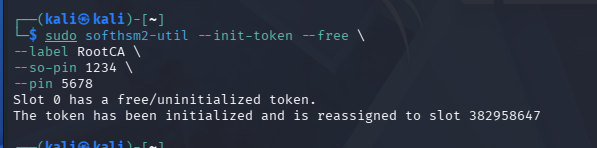
\includegraphics[width=0.82\linewidth]{images/win_hsm_init_token.png}
  \caption{Initialisation du token SoftHSM2 \texttt{RootCA} : le slot libre est initialisé
  et réassigné.}
  \label{fig:hsm-init}
\end{figure}
\begin{figure}[htbp]
  \centering
  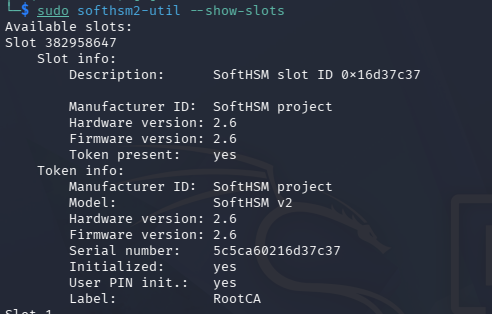
\includegraphics[width=0.62\linewidth]{images/win_hsm_slots.png}
  \caption{\texttt{softhsm2-util --show-slots} : le token \texttt{RootCA} est présent,
  initialisé, PIN utilisateur défini (SoftHSM v2).}
  \label{fig:hsm-slots}
\end{figure}

\subsubsection{Clé RSA 4096 dans le token et racine auto-signée}
La bi-clé RSA 4096 est créée dans le token, puis OpenSSL~3 auto-signe le certificat racine
en accédant à la clé privée \emph{via le provider} \texttt{pkcs11prov} (la clé n'est jamais
copiée sur le disque) :
\begin{lstlisting}[style=cmd]
openssl req -provider default -provider pkcs11prov \
  -new -x509 -days 3650 -sha256 \
  -subj "/C=FR/O=TP Crypto/CN=TP Root CA" \
  -key "$ROOT_KEY_URI" \
  -addext "basicConstraints=critical,CA:TRUE" \
  -addext "keyUsage=critical,cRLSign,keyCertSign" \
  -addext "subjectKeyIdentifier=hash" \
  -addext "authorityKeyIdentifier=keyid:always" \
  -out certs/rootCA.crt
\end{lstlisting}
\begin{figure}[htbp]
  \centering
  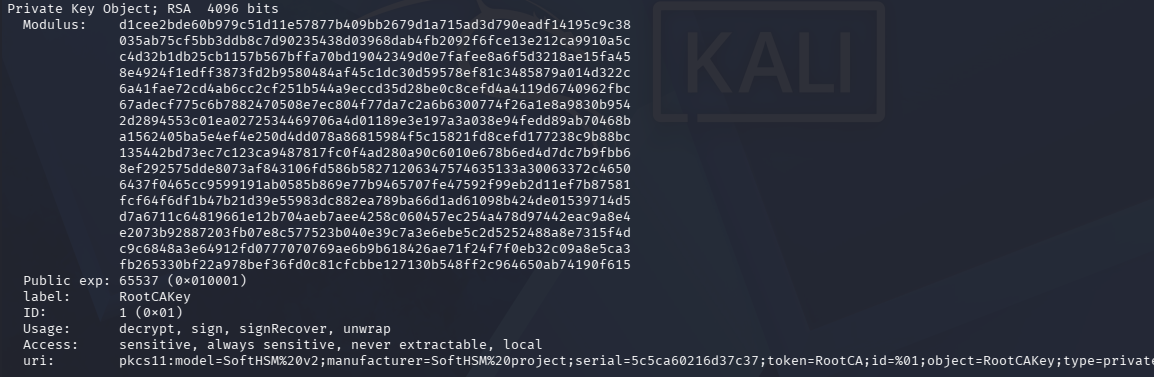
\includegraphics[width=0.62\linewidth]{images/win_hsm_root_req.png}
  \caption{Création/auto-signature de la racine via PKCS\#11 : OpenSSL retrouve bien la clé
  privée \texttt{RootCAKey} dans le token \texttt{RootCA} (module \texttt{p11-kit-proxy.so}).}
  \label{fig:hsm-root-req}
\end{figure}

\noindent Le certificat racine obtenu est bien une RSA 4096 bits, auto-signée, avec les
extensions d'une AC :
\begin{figure}[htbp]
  \centering
  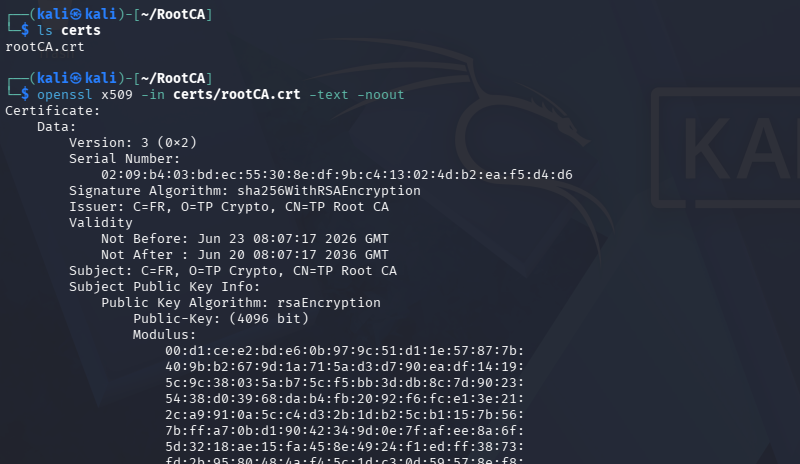
\includegraphics[width=0.7\linewidth]{images/win_hsm_root_cert.png}
  \caption{\texttt{openssl x509 -text} sur \texttt{certs/rootCA.crt} : RSA 4096 bits,
  sujet et émetteur identiques (\texttt{O=TP Crypto, CN=TP Root CA}), validité 10 ans.}
  \label{fig:hsm-root-cert}
\end{figure}
\begin{figure}[htbp]
  \centering
  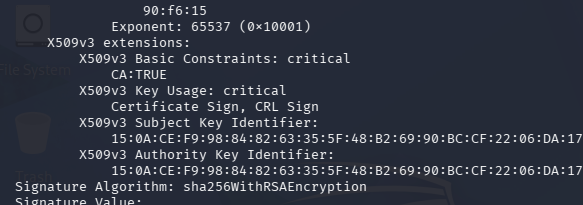
\includegraphics[width=0.7\linewidth]{images/win_hsm_root_ext.png}
  \caption{Extensions de la racine : \texttt{Basic Constraints CA:TRUE} (critique),
  \texttt{Key Usage : Certificate Sign, CRL Sign}.}
  \label{fig:hsm-root-ext}
\end{figure}

\begin{notebox}
La racine a été régénérée en fin de manipulation sous le \emph{Common Name} \texttt{RootCA}
(mêmes paramètres : \texttt{O=TP Crypto}, RSA 4096) ; c'est cette dernière, visible plus
loin dans le magasin Windows, qui a signé l'AC subordonnée ADCS. Les captures de cette
sous-section illustrent la racine SoftHSM2 dans sa première version (\texttt{TP Root CA}).
\end{notebox}

\subsection{CRL / ARL de la racine HSM}
La racine publie une CRL (qui sert ici d'ARL puisqu'elle ne signe que des AC) valable
un mois et, pour l'instant, sans certificat révoqué :
\begin{figure}[htbp]
  \centering
  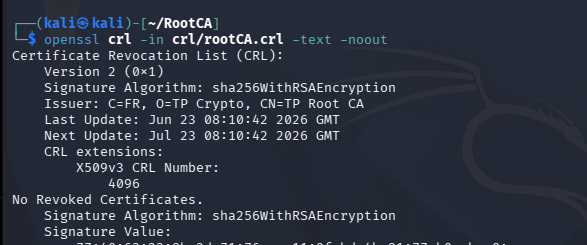
\includegraphics[width=0.72\linewidth]{images/win_hsm_crl.png}
  \caption{CRL de la racine SoftHSM2 : \texttt{Last/Next Update} espacés d'un mois,
  \texttt{No Revoked Certificates}.}
  \label{fig:hsm-crl}
\end{figure}

\subsection{Absence d'export de clé privée}
On vérifie qu'aucun fichier de clé privée (\fichier{.key} ou \fichier{.pem} privé) n'a été
écrit hors du token : la recherche ne renvoie rien, ce qui confirme que la clé reste
confinée dans SoftHSM2.
\begin{figure}[htbp]
  \centering
  
\includegraphics[width=0.6\linewidth]{images/win_hsm_nokey.png}
  \caption{\texttt{find . -type f | grep -E "\textbackslash.key|\textbackslash.pem"} ne
  retourne aucun fichier : aucune clé privée exportée hors du HSM.}
  \label{fig:hsm-nokey}
\end{figure}

\subsection{Point technique PKCS\#11}
Le moteur (\emph{engine}) historique \texttt{pkcs11} est bien listé comme disponible par
OpenSSL, mais l'ancienne syntaxe \cmdinline{openssl x509 -req -engine pkcs11} échoue sous
OpenSSL~3 (« \texttt{bad engine id} », clé privée PKCS\#11 introuvable). La solution
retenue est le \emph{provider} OpenSSL~3 \texttt{pkcs11prov}, utilisé pour toutes les
opérations de signature ci-dessus et ci-dessous.
\begin{figure}[htbp]
  \centering
  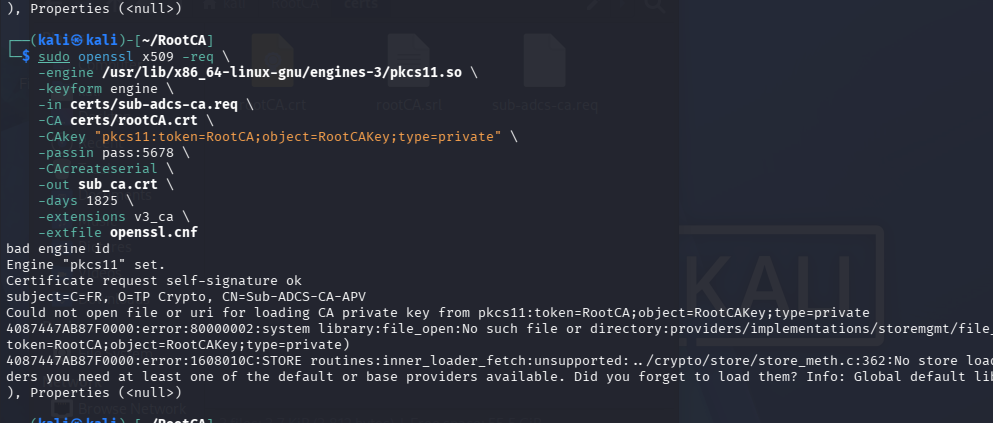
\includegraphics[width=0.78\linewidth]{images/win_pkcs11_engine_fail.png}
  \caption{Échec de la voie \emph{engine} (\texttt{-engine pkcs11}) : « bad engine id »
  et impossibilité de charger la clé privée PKCS\#11. La signature passera par le
  \emph{provider} \texttt{pkcs11prov}.}
  \label{fig:pkcs11-fail}
\end{figure}

\subsection{Autorité subordonnée ADCS Windows}
\label{sec:adcs}

\subsubsection{Objectif et vocabulaire}
La dernière étape consiste à faire d'un \textbf{Windows Server 2019} une AC subordonnée
de notre racine HSM Linux. Autrement dit, la clé privée de cette sous-AC est générée et
conservée sur Windows, mais son certificat est signé par la racine
\texttt{HSM\_Root\_CA\_TRI} restée côté Linux/SoftHSM2. On obtient une chaîne hétérogène
Linux~$\rightarrow$~Windows, ce qui illustre l'interopérabilité du standard X.509.

\noindent Quelques termes Microsoft à connaître :
\begin{itemize}[leftmargin=1.4em]
  \item \textbf{ADCS} (\emph{Active Directory Certificate Services}) : le rôle Windows
  qui fournit une autorité de certification. Le service système correspondant s'appelle
  \texttt{CertSvc}.
  \item \textbf{Standalone} (autonome) vs \textbf{Enterprise} : une AC \emph{Enterprise}
  s'intègre à un annuaire Active Directory (gabarits, auto-enrôlement). Une AC
  \emph{Standalone} est indépendante de tout domaine ; c'est ce que demande le TP, car la
  VM n'est pas contrôleur de domaine.
  \item \textbf{Subordinate} (subordonnée) vs \textbf{Root} : une AC \emph{Root} s'auto-signe ;
  une AC \emph{Subordinate} génère une \emph{CSR} (PKCS\#10) qu'une autorité parente doit
  signer. Ici l'autorité parente est notre racine SoftHSM2 Linux.
\end{itemize}

\begin{notebox}
\textbf{Nom de l'AC.} Le nom logique du TP est « APV », mais ADCS gère mal les
soulignés (\texttt{\_}) dans le \emph{Common Name} d'une AC (problèmes d'encodage
ASN.1/Unicode). On a donc normalisé le nom Windows en \texttt{Sub-ADCS-CA-APV} (avec des
tirets). C'est purement cosmétique et n'affecte pas la cryptographie.
\end{notebox}

Toute la procédure est automatisée par le script \fichier{windows-adcs/run-on-windows.ps1} les commandes ci-dessous sont celles qu'il exécute, détaillées pour le
compte rendu. Le déroulement est en \textbf{deux passages} sur Windows, séparés par une
signature côté Linux.

\subsubsection{Premier passage Windows : rôle ADCS et génération de la CSR}
On copie le dossier \fichier{windows-adcs} sur le Bureau de l'administrateur, puis dans une
console \textbf{PowerShell ouverte en administrateur} :
\begin{lstlisting}[style=cmd]
cd C:\Users\Administrateur\Desktop\windows-adcs
Set-ExecutionPolicy -Scope Process -ExecutionPolicy Bypass -Force
.\run-on-windows.ps1            # ajouter -ResetADCS si une VM a deja servi
\end{lstlisting}
Ce passage exécute pour l'essentiel :
\begin{lstlisting}[style=cmd]
# 1) Installer le role d'autorite de certification
Install-WindowsFeature -Name ADCS-Cert-Authority -IncludeManagementTools

# 2) Creer une AC subordonnee AUTONOME : cle RSA 4096 + SHA-256,
#    et produire la CSR a faire signer par la racine Linux.
Install-AdcsCertificationAuthority `
  -CAType StandaloneSubordinateCA `
  -CACommonName "Sub-ADCS-CA-APV" `
  -CADistinguishedNameSuffix "O=TP Crypto, C=FR" `
  -CryptoProviderName "RSA#Microsoft Software Key Storage Provider" `
  -KeyLength 4096 `
  -HashAlgorithmName SHA256 `
  -OutputCertRequestFile C:\TP-Crypto-ADCS\output\sub-adcs-ca.req `
  -IgnoreUnicode -Force
\end{lstlisting}
\begin{notebox}
On ne précise volontairement \emph{pas} \texttt{-ValidityPeriod} ici : pour une AC
\emph{subordonnée}, la durée de validité est imposée par l'autorité parente au moment où
elle signe la CSR (côté Linux, on signera pour 5~ans). C'est normal que le service
\texttt{CertSvc} ne démarre pas encore : il manque le certificat signé.
\end{notebox}
\begin{reponse}
Le rôle \emph{Autorité de certification} (\texttt{ADCS-Cert-Authority}) est bien installé
(figure~\ref{fig:adcs-feature}) et le fichier
\fichier{C:\textbackslash TP-Crypto-ADCS\textbackslash output\textbackslash sub-adcs-ca.req}
(requête PKCS\#10, figure~\ref{fig:adcs-csr}) est créé. Le script invite alors à le faire
signer côté Linux.
\end{reponse}
\begin{figure}[htbp]
  \centering
  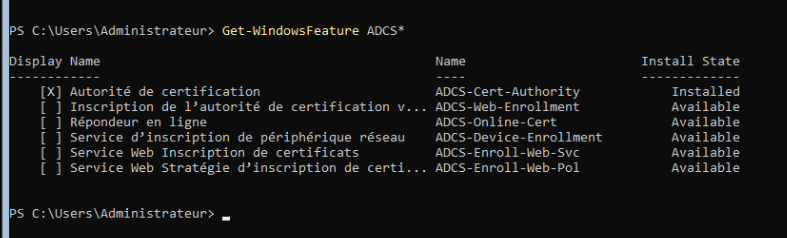
\includegraphics[width=0.85\linewidth]{images/win_adcs_feature.png}
  \caption{\texttt{Get-WindowsFeature ADCS*} : le rôle \emph{Autorité de certification}
  (\texttt{ADCS-Cert-Authority}) est à l'état \texttt{Installed}.}
  \label{fig:adcs-feature}
\end{figure}
\begin{figure}[htbp]
  \centering
  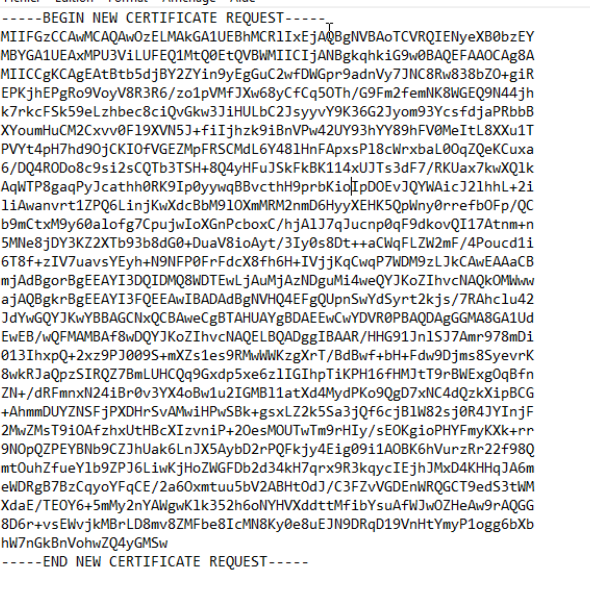
\includegraphics[width=0.55\linewidth]{images/win_adcs_csr.png}
  \caption{La requête PKCS\#10 de l'AC subordonnée (\texttt{-----BEGIN NEW CERTIFICATE
  REQUEST-----}) générée par ADCS, à transmettre à la racine Linux.}
  \label{fig:adcs-csr}
\end{figure}

\subsubsection{Signature de la CSR côté Linux (racine SoftHSM2)}
On rapatrie \fichier{sub-adcs-ca.req} sur le poste Linux, puis on la signe avec la clé de
la racine restée dans le HSM, toujours via le provider \texttt{pkcs11prov} (la clé privée
n'est jamais exportée) :
\begin{lstlisting}[style=cmd]
openssl x509 -req -provider default -provider pkcs11prov \
  -in certs/sub-adcs-ca.req \
  -CA certs/rootCA.crt \
  -CAkey "pkcs11:token=RootCA;object=RootCAKey;type=private;pin-value=5678" \
  -CAcreateserial -days 1825 \
  -extensions v3_ca -extfile openssl.cnf \
  -out sub_ca.crt
\end{lstlisting}
Le profil d'extensions appliqué (\texttt{v3\_ca}) fait bien de la cible une AC subordonnée :
\begin{lstlisting}[style=conf]
[v3_ca]
basicConstraints       = critical, CA:true
keyUsage               = critical, digitalSignature, cRLSign, keyCertSign
subjectKeyIdentifier   = hash
authorityKeyIdentifier = keyid:always,issuer
\end{lstlisting}
\begin{notebox}
\texttt{-days 1825} fixe la validité de l'AC subordonnée à 5~ans : c'est bien la racine
parente qui décide de la durée, comme annoncé au premier passage Windows.
\end{notebox}
\begin{reponse}
Le certificat \fichier{sub\_ca.crt} obtenu est émis par \texttt{CN=RootCA} pour le sujet
\texttt{CN=Sub-ADCS-CA-APV, O=TP Crypto, C=FR}, valable du 23/06/2026 au 22/06/2031
(5~ans) — voir la vérification figure~\ref{fig:adcs-verify}.
\end{reponse}

\subsubsection{Second passage Windows : import de la racine et finalisation}
On recopie côté Windows le certificat signé \fichier{sub\_ca.crt} \emph{et} le certificat
racine \fichier{rootCA.crt}, puis on importe la racine comme ancre de confiance et on
installe le certificat de la sous-AC :
\begin{lstlisting}[style=cmd]
# Importer la racine Linux comme ancre de confiance (cf. tache 15)
certutil -addstore Root  C:\TP-Crypto-ADCS\input\rootCA.crt
# Installer le certificat signe dans l'AC subordonnee, puis demarrer le service
certutil -installCert C:\TP-Crypto-ADCS\input\sub_ca.crt
Start-Service CertSvc
\end{lstlisting}
La racine SoftHSM2 est alors bien présente dans le magasin
\emph{Autorités de certification racines de confiance} de la machine
(figure~\ref{fig:adcs-rootstore}).
\begin{figure}[htbp]
  \centering
  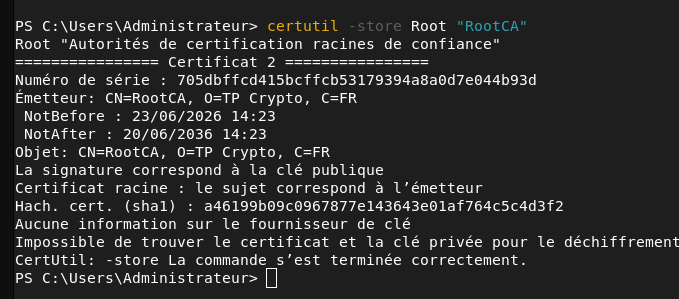
\includegraphics[width=0.78\linewidth]{images/win_adcs_rootstore.png}
  \caption{\texttt{certutil -store Root "RootCA"} : la racine SoftHSM2 (\texttt{CN=RootCA,
  O=TP Crypto}) est installée comme ancre de confiance, « le sujet correspond à
  l'émetteur » (racine auto-signée).}
  \label{fig:adcs-rootstore}
\end{figure}

\subsubsection{Vérification de la chaîne hétérogène Linux $\rightarrow$ Windows}
C'est le résultat central de la Partie~3 : le certificat de l'AC subordonnée, hébergée sous
Windows, se valide jusqu'à la racine SoftHSM2 importée.
\begin{lstlisting}[style=cmd]
certutil -verify -urlfetch .\sub_ca.crt
\end{lstlisting}
\begin{figure}[htbp]
  \centering
  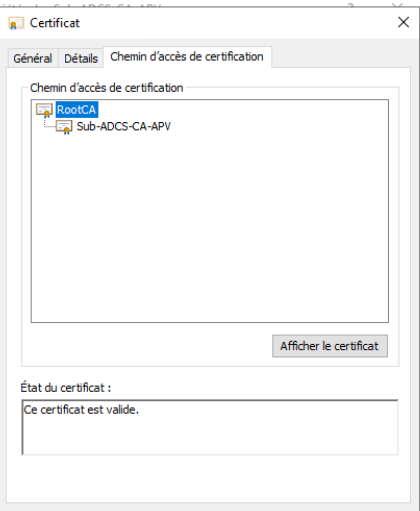
\includegraphics[width=0.66\linewidth]{images/win_adcs_chain.png}
  \caption{Onglet \emph{Chemin d'accès de certification} : la chaîne \texttt{RootCA}
  $\rightarrow$ \texttt{Sub-ADCS-CA-APV} est complète et « Ce certificat est valide ».}
  \label{fig:adcs-chain}
\end{figure}
\begin{figure}[htbp]
  \centering
  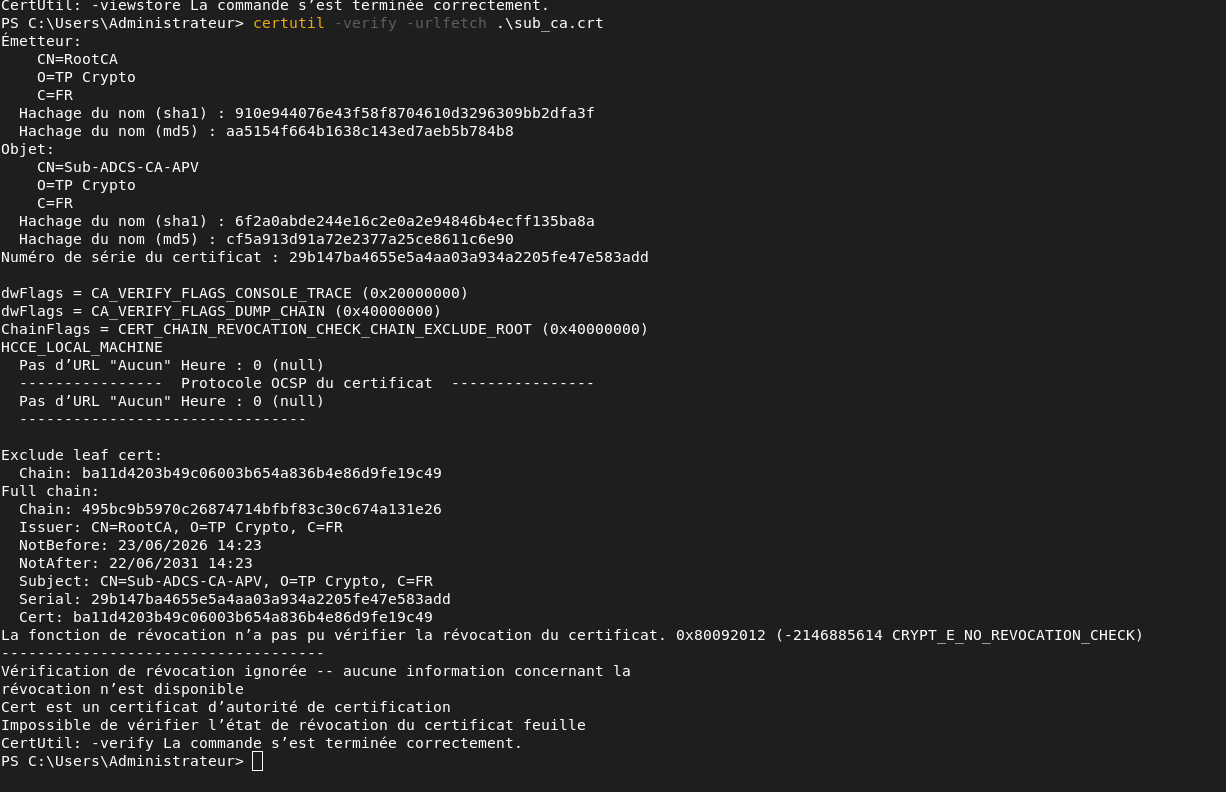
\includegraphics[width=0.92\linewidth]{images/win_adcs_verify.png}
  \caption{\texttt{certutil -verify} sur \texttt{sub\_ca.crt} : émetteur \texttt{CN=RootCA},
  sujet \texttt{CN=Sub-ADCS-CA-APV}, validité 23/06/2026 → 22/06/2031, chaîne complète
  reconstruite jusqu'à la racine. La seule remarque (\texttt{CRYPT\_E\_NO\_REVOCATION\_CHECK})
  est normale : aucune URL de CRL/OCSP en ligne pour cette racine de TP.}
  \label{fig:adcs-verify}
\end{figure}
\begin{reponse}
La chaîne \texttt{Sub-ADCS-CA-APV} $\rightarrow$ \texttt{RootCA} est validée par Windows
(« Ce certificat est valide », figure~\ref{fig:adcs-chain}). Windows fait donc confiance à
une AC dont l'ancre est une racine dont la \textbf{clé privée n'a jamais quitté le HSM
SoftHSM2 sous Linux}. L'objectif d'interopérabilité Linux/Windows autour d'une racine
adossée à un HSM est atteint. Le seul avertissement de \texttt{certutil -verify} porte sur
l'absence de point de révocation en ligne, attendu pour une PKI de laboratoire hors ligne.
\end{reponse}

\subsubsection{Émission d'un certificat TLS par l'AC ADCS}
Une fois l'AC subordonnée opérationnelle (\texttt{CertSvc} en \texttt{Running}), elle peut
émettre des certificats d'entité finale. On génère une CSR TLS à partir d'un fichier
\fichier{.inf}, puis on la soumet à l'AC :
\begin{lstlisting}[style=cmd]
# CSR TLS depuis le modele .inf (RSA 3072, EKU serverAuth, SAN dns=www.tp-crypto.local)
certreq -new    C:\TP-Crypto-ADCS\output\web-tls.inf C:\TP-Crypto-ADCS\output\web-tls.req
certreq -submit -config "$env:COMPUTERNAME\Sub-ADCS-CA-APV" `
  C:\TP-Crypto-ADCS\output\web-tls.req C:\TP-Crypto-ADCS\output\web-tls.cer
\end{lstlisting}
\begin{notebox}
Une AC \emph{Standalone} met par défaut les demandes \emph{en attente} : le script les
valide automatiquement (\cmdinline{certutil -resubmit} puis \cmdinline{certreq -retrieve}).
Le certificat émis porte alors l'EKU \emph{TLS Web Server Authentication} et le SAN
\texttt{DNS:www.tp-crypto.local}, et se vérifie avec \cmdinline{certutil -verify
web-tls.cer}. Tous les artefacts et journaux sont regroupés dans
\fichier{C:\textbackslash TP-Crypto-ADCS\textbackslash} (rapport
\fichier{RAPPORT-WINDOWS-ADCS.md} et dossier \fichier{logs\textbackslash}).
\end{notebox}

\end{document}
